% $Id: SolarSystem.tex,v 1.1 2008/01/31 18:04:17 dconway Exp $
\chapter{\label{chapter:SolarSystem}The Space Environment}
\chapauthor{Darrel J. Conway}{Thinking Systems, Inc.}

The core purpose of GMAT is to perform flight dynamics simulations for spacecraft flying in the
solar system.  There are many different components that users interact with to produce this model.
In this chapter, the architecture for the elements that comprise the model is introduced.  The
elements that are not directly manipulated in the model -- specifically, the Sun, planets, moons,
and related points that comprise the stage on which the spacecraft and related objects perform
their actions -- are described in some detail in the chapter.  Descriptions for the other objects
-- most specifically spacecraft and formations -- introduced here appear in chapters for those
components.  References for those chapters are provided when the objects are introduced.

\section{Components of the Model}

The environmental elements that have a spatial location and evolve over time in the GMAT model are
all derived from the SpacePoint class.  The class hierarchy, shown in
Figure~\ref{figure:EnvironmentalObjects}, includes classes that model the objects and
special locations in GMAT's solar system -- referred to as ``background'' objects because their
evolution is modeled through precalculated ephemerides or computations performed off of these
precalculated data -- along with the pieces that are directly manipulated in the mission control
sequence and that evolve through numerical integration using GMAT's propagation subsystem.  In the
figure, the classes used to model background objects are shown in purple; those that evolve through
direct modeling in GMAT using the propagation subsystem are shown in blue, and other elements that
will be incorporated in the future, in red.

\begin{figure}[htb]
\begin{center}
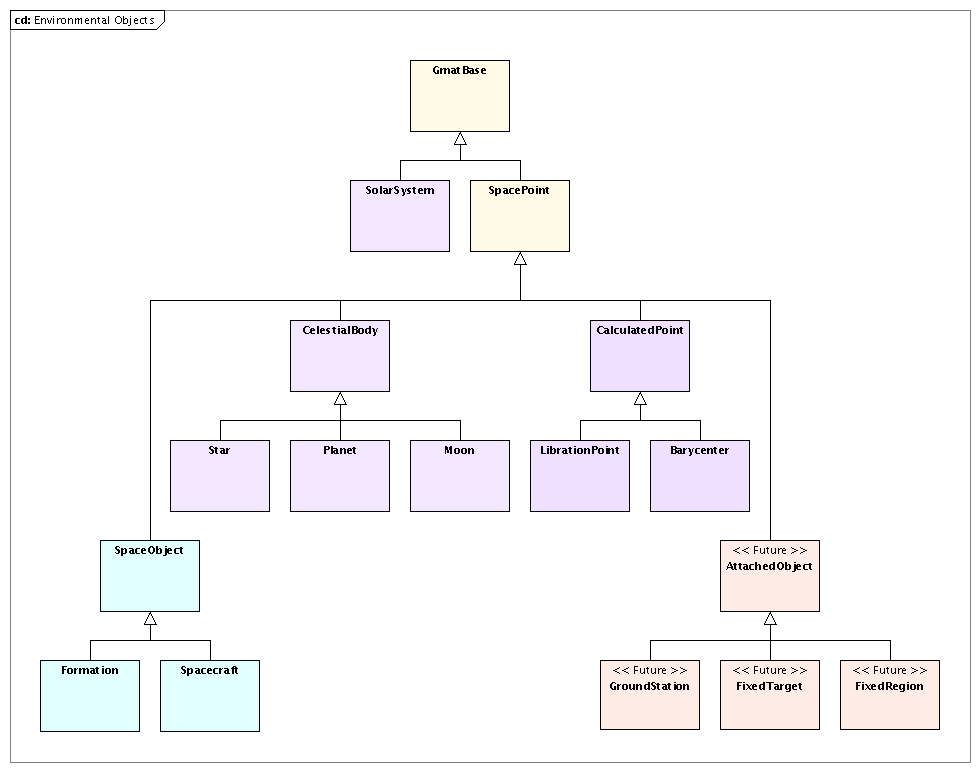
\includegraphics[440,347]{Images/EnvironmentalObjects.png}
\caption[Objects in the GMAT Model]{\label{figure:EnvironmentalObjects}Objects in the GMAT
Model.\\The elements shown in purple are core constituents of GMAT's solar system.  Classes
shown in yellow are GMAT base classes.  Elements shown in blue are the key components
studied in GMAT's model: Spacecradft and Formations of Spacecraft.  Those shown in red are future
enhancements, primarily focussed on contact analysis with different types of objects.}
\end{center}
\end{figure}

The space environment as defined in this document consists of the elements that, while dynamic, are
automatically updated as the model evolves, based on epoch data generated for the model.  These
elements are the gravitating bodies in the model -- that is, the Sun and the planets and their moons
-- and points with specialized significance in flight dynamics, like the Lagrange points and
gravitational barycenters.  All of these elements are managed in an instance of the SolarSystem
class. SolarSystem acts as a container, and manages both the objects in the space environment and
the resources needed to calculate ephemerides for these objects.  The bulk of this chapter provides
details about the classes and objects comprising this space environment.

A key feature of GMAT is the ability to model spacecraft and formations of spacecraft as they move
through the space environment.  These elements of the model are configured in detail by GMAT users,
and evolve through time using precision numerical integrators configured by the users.  The
Spacecraft and Formation classes, along with their base SpaceObject class, are discussed in detail
in Chapter~\ref{chapter:Spacecraft}.  The numerical integrators and associated force model
components are presented in Chapter~\ref{chapter:Propagators}.

The class hierarchy includes provisions for future model elements attached to components of the
space environment.  These classes, FixedObject and the derived GroundStation, FixedTarget and
FixedRegion classes, will be documented at a later date in preparation for implementation.

Before proceeding with a detailed description of GMAT's space environment, the base class used for
all of the model elements needs some explanation.  Those details are provided in the next section.

\section{\label{section:SpacePoint}The SpacePoint Class}

All spatially modeled components need some common data in order to define the positions of objects
in the model.  These data are collected in the SpacePoint base class.  This base class provides the
foundation for objects used to define coordinate systems (see
Chapter~\ref{chapter:CoordinateSystems}), for the user configured Spacecraft and Formations (see
Chapter~\ref{chapter:Spacecraft}), and for other specialized points and objects in the space
environment.

\begin{figure}[htb]
\begin{center}
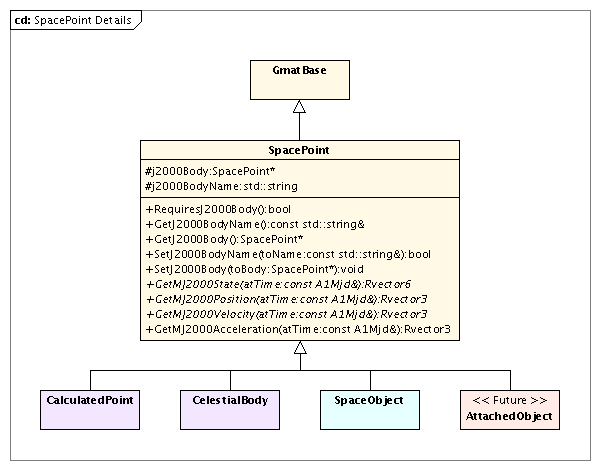
\includegraphics[300,235]{Images/SpacePointDetails}
\caption{\label{figure:SpacePointDetails}The SpacePoint Class}
\end{center}
\end{figure}

Figure~\ref{figure:SpacePointDetails} shows the elements of the SpacePoint class.  In
order for GMAT to accurately model flight dynamics problems, the GMAT space model needs to specify
an internal origin and coordinate system orientation used as a reference for computations.
SpacePoint defines one object, the J2000 body, which is used to define that origin.  GMAT uses the
Mean-of-J2000 Earth Equatorial axis system as the orientation for all such calculations.

\subparagraph{\textit{Class Attributes}}

SpacePoint defines two data members to track the J2000 body:

\begin{itemize}
\item \textbf{SpacePoint* j2000Body}: The body used to define the coordinate origin for the
SpacePoint.
\item \textbf{std::string j2000BodyName}: The name of the body defining the coordinate origin.
\end{itemize}

\subparagraph{\textit{Methods}}

All classes derived from SpacePoint inherit the implementation of six methods used to set and access
the J2000 body.  Five of these methods are used specifically for the internal data members; the
sixth, GetMJ2000Acceleration(), provides a default implementation so that derived classes that do
not have acceleration data do not need to provide an implementation

\begin{itemize}
\item \textbf{bool RequiresJ2000Body()}: Returns a boolean used to determine if the SpacePoint
requires a J2000 body.
\item \textbf{const std::string\& GetJ2000BodyName()}: Returns the name of the J2000 body for the
SpacePoint.
\item \textbf{SpacePoint *GetJ2000Body()}: Returns the pointer to the J2000 body for the
SpacePoint.
\item \textbf{bool SetJ2000BodyName(const std::string \&toName)}: Sets the name of the J2000 body
for the SpacePoint.
\item \textbf{void SetJ2000Body(SpacePoint *toBody)}: Sets the pointer to the J2000 body for the
SpacePoint.
\item \textbf{Rvector3 GetMJ2000Acceleration(const A1Mjd \&atTime)}: Returns the Cartesian
acceleration of the SpacePoint relative to its J2000 body at the specified epoch.  The default
implementation returns [0.0, 0.0, 0.0]; derived classes that contain acceleration data should
override this method.
\end{itemize}

\subparagraph{\textit{Abstract Methods}}

Each subclass of SpacePoint implements three pure virtual methods defined in the class, using
computations specific to that subclass.  THese abstract methods have the following signatures:

\begin{itemize}
\item \textbf{virtual Rvector6 GetMJ2000State(const A1Mjd \&atTime) = 0}: Returns the Cartesian
state of the SpacePoint relative to its J2000 body at the specified epoch.
\item \textbf{virtual Rvector3 GetMJ2000Position(const A1Mjd \&atTime) = 0}: Returns the Cartesian
location of the SpacePoint relative to its J2000 body at the specified epoch.
\item \textbf{virtual Rvector3 GetMJ2000Velocity(const A1Mjd \&atTime) = 0}: Returns the Cartesian
velocity of the SpacePoint relative to its J2000 body at the specified epoch.
\end{itemize}

\section{The Solar System Elements}

GMAT provides a container class, SolarSystem, that is used to manage the objects modeling the space
environment.

\subsection{The SolarSystem Class}

\subsubsection{Members and Methods}

\subsubsection{Ephemeris Sources}

\subsection{The CelestialBody Class Hierarchy}

\subsubsection{Stars}

\subsubsection{Planets}

\subsubsection{Moons}

\section{The PlanetaryEphem Class}

